%label:"art:RationalEquivalenceInTropicalGeometry"
%type:"article"
%name:"rational equivalence in tropical geometry"
%caption:""
%parent:"art_TropicalChowGroupsII"


%label:"def:TropicalRationalEquivalence"
%type:"definition"
%name:"tropical rational equivalence"
%caption:""
%parent:"art_RationalEquivalenceInTropicalGeometry"


    Let $Z\subset Q$ be a subcycle (bounded) rationally equivalent to $0$ if there exists a cycle $Y, \dim(Y)=\dim(Z)$ and a morphism $Y\to Q$ and a (bounded) rational function $\phi\in \mathcal K^*_Y$ such that 
    \[f_*(\deg(\phi)\cdot Y)=Z.\]


If you're familiar with rational equivalence in algebraic geometry, the main difference is that we ask the cycle $Y$ to be a subvariety of $X$. Originally, the definition used that $Y$ was a subset of $X$, but unfortunately this definition is not compatible with pushforward. The belief is that the definition of tropical rational function is too rigid (so our definition for tropical rational equivalence) is a bit more flexible. 
%label:"def:TropicalChowGroup"
%type:"definition"
%name:"tropical chow group"
%caption:""
%parent:"art_RationalEquivalenceInTropicalGeometry"


    Let $X$ be a tropical variety. We define the tropical chow groups $A^{(b)}_\bullet(X)=Z^{(b)}_\bullet(X)/\sim^{(b)}$


     Let $Q\subset Q\times \RR$. Let $\phi_p$ be the pullback of $\max(x, p')$. 
    Then $F_p=\mathrm{Div}(\phi\cdot F)\subset Q\times \{Q\}\cong Q$
Given $P_1, 2\in Q$ we say that the are $\sim^\RR$ if there exists a cycle $F$ and points $q_1, q_2\in \RR$ so that $P_i=F_{q_i}$. 
%label:"prp:CharacterizationOfBoundedRationalEquiavlence"
%type:"proposition"
%name:"characterization of bounded rational equiavlence"
%caption:""
%parent:"art_RationalEquivalenceInTropicalGeometry"


    A cycle $P_1\sim^b 0$ if and only if $Z_1\sim^\RR 0$


%label:"prf:CharacterizationOfBoundedRationalEquiavlence"
%type:"proof"
%name:"characterization of bounded rational equiavlence"
%caption:""
%parent:""


    Suppose that $P_1\sim^\RR P_2$. Then there exists $F\subset Q\times \RR$ with $F_{q_i}=P_i$. 

    Take $R=F$, and define $\phi:=\pi^*\psi$. We see that $(\pi_Q)_* (\pi^*(\psi^*\psi)\cdot F)=P_1-P_2$. 

    NOw suppose instead that $P_1\sim^b P_2$. Then there exists $R$ and $\phi\in \mathcal K_R$ such that $f_*(\mathrm{Div}(\phi))=P_1-P_2$. 
    Tke $F:=(f\times \id)_* (\text{graph}(\phi))$. Cruicially, the function $\phi$ is bounded so that the intersection with a sufficiently large slice is empty 
%label:"fig:ALargeSliceIsEmpty"
%type:"figure"
%name:"a large slice is empty"
%caption:"sufficiently large slices have empty intersection"
%parent:"prf_CharacterizationOfBoundedRationalEquiavlence"


        \begin{tikzpicture}

            \draw (-1.5,0) -- (1.5,0);
            \draw (-1.5,0.5) -- (-0.5,0.5) -- (0.5,2) -- (1.5,2);
            \node at (2.5,0) {$R$};
            \draw (-0.5,0.5) -- (-0.5,-0.5) (0.5,2) -- (0.5,-0.5);
            \draw[dashed] (-1.5,-0.5) -- (1.5,-0.5);
            \draw[dashed] (-1.5,3) -- (1.5,3);
            \end{tikzpicture}




\begin{remark}
    Observe that if $R\subset P$ has $R\sim^b 0$ and $g: P\to Q$ is a map of tropical varities that $g_*Z\sim^b0$. However, consider the morphism 
    this gives an example of $Z\sim 0$ but $f_*Z\not\sim 0$. 
%label:"fig:APullbackOfAZeroCycleMayNotBeZero"
%type:"figure"
%name:"a pullback of a zero cycle may not be zero. "
%caption:""
%parent:"art_RationalEquivalenceInTropicalGeometry"


        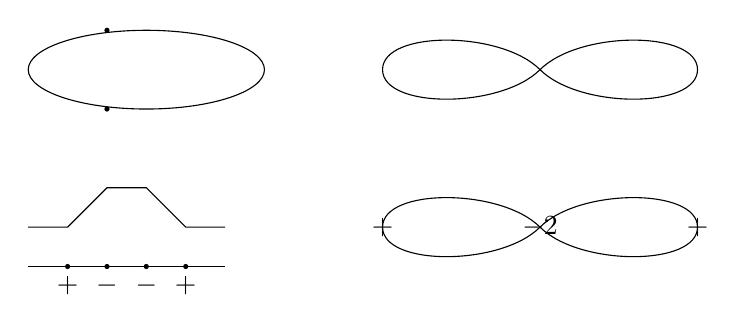
\begin{tikzpicture}


            \draw  (-2.5,0.5) ellipse (1.5 and 0.5);
            \draw (2.5,0.5) .. controls (2,0) and (0.5,0) .. (0.5,0.5) .. controls (0.5,1) and (2,1) .. (2.5,0.5) .. controls (3,0) and (4.5,0) .. (4.5,0.5) .. controls (4.5,1) and (3,1) .. (2.5,0.5);
            \node[circle, scale=.2, fill] at (-3,1) {};
            \node[circle, scale=.2, fill] at (-3,0) {};
            \draw (-4,-2) -- (-1.5,-2);
            \draw (-4,-1.5) -- (-3.5,-1.5) -- (-3,-1) -- (-2.5,-1) -- (-2,-1.5) -- (-1.5,-1.5);
            \node[circle, scale=.2, fill] at (-3.5,-2) {};
            \node[circle, scale=.2, fill] at (-3,-2) {};
            \node[circle, scale=.2, fill] at (-2,-2) {};
            \node[circle, scale=.2, fill] at (-2.5,-2) {};
            
            
            \node[below] at (-3.5,-2) {$+$};
            \node[below] at (-3,-2) {$-$};
            \node[below] at (-2,-2) {$+$};
            \node[below] at (-2.5,-2) {$-$};
            
            \begin{scope}[shift={(0,-2)}]
            \draw (2.5,0.5) .. controls (2,0) and (0.5,0) .. (0.5,0.5) .. controls (0.5,1) and (2,1) .. (2.5,0.5) .. controls (3,0) and (4.5,0) .. (4.5,0.5) .. controls (4.5,1) and (3,1) .. (2.5,0.5);
            
            \end{scope}
            
            \node at (0.5,-1.5) {$+$};
            \node at (4.5,-1.5) {$+$};
            \node at (2.5,-1.5) {$-2$};
            \end{tikzpicture}


\end{remark}

